\section{Python Parse Error Analysis}
\label{sec:error-analysis}

We perform here an \emph{error data analysis} on a \python dataset of more than
\emph{1,100,000 erroneous Python programs} and their respective fixes. This
dataset was gathered from PythonTutor.com~\citep{Guo2013} between the years 2017
and 2018, previously used in related work \citep{Endres2019, Cosman2020}. Each
program which throws an uncaught \python exception is paired with the next
program by the same user that does not crash, under the assumption that the
latter is the fixed version of the former. We discard pairs where the difference
between crashing and fixed versions is too high (more than a standard deviation
above average), since these are usually unrelated submissions or complete
refactorings. We also discard submissions that violate PythonTutor's policies
(e.g., those using forbidden libraries). Ultimately, the dataset used in this
evaluation contains more than a million usable program pairs, representing
students from dozens of universities (PythonTutor has been used in many
introductory courses~\citep{Guo2013}) as well as non-traditional novices.

\begin{figure}[t]
  \centering
  \begin{minipage}[c]{0.51\linewidth}
    \centering
    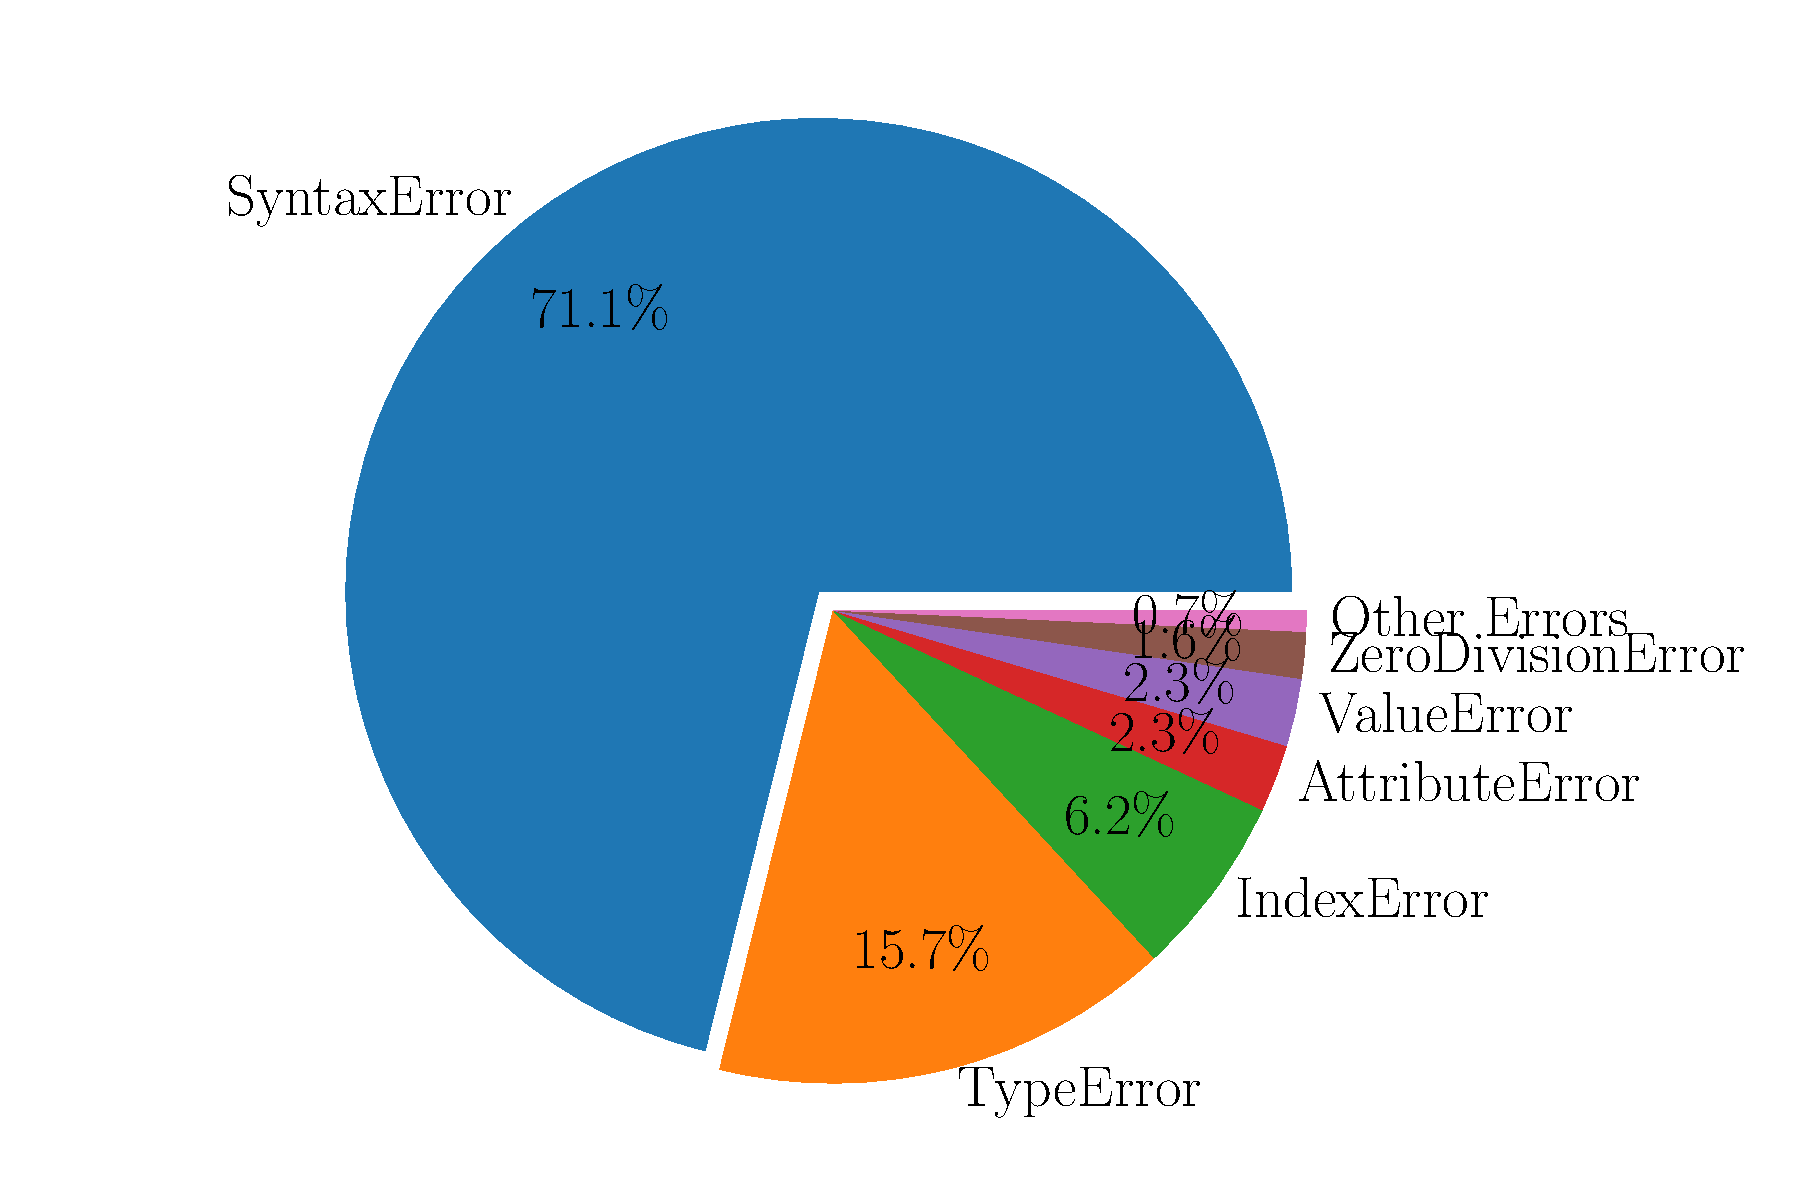
\includegraphics[width=\linewidth]{error-pie.pdf}
    \caption{The Python error type distribution.}
    \label{fig:error-statistics}
  \end{minipage}
  \begin{minipage}[c]{0.48\linewidth}
      \centering
      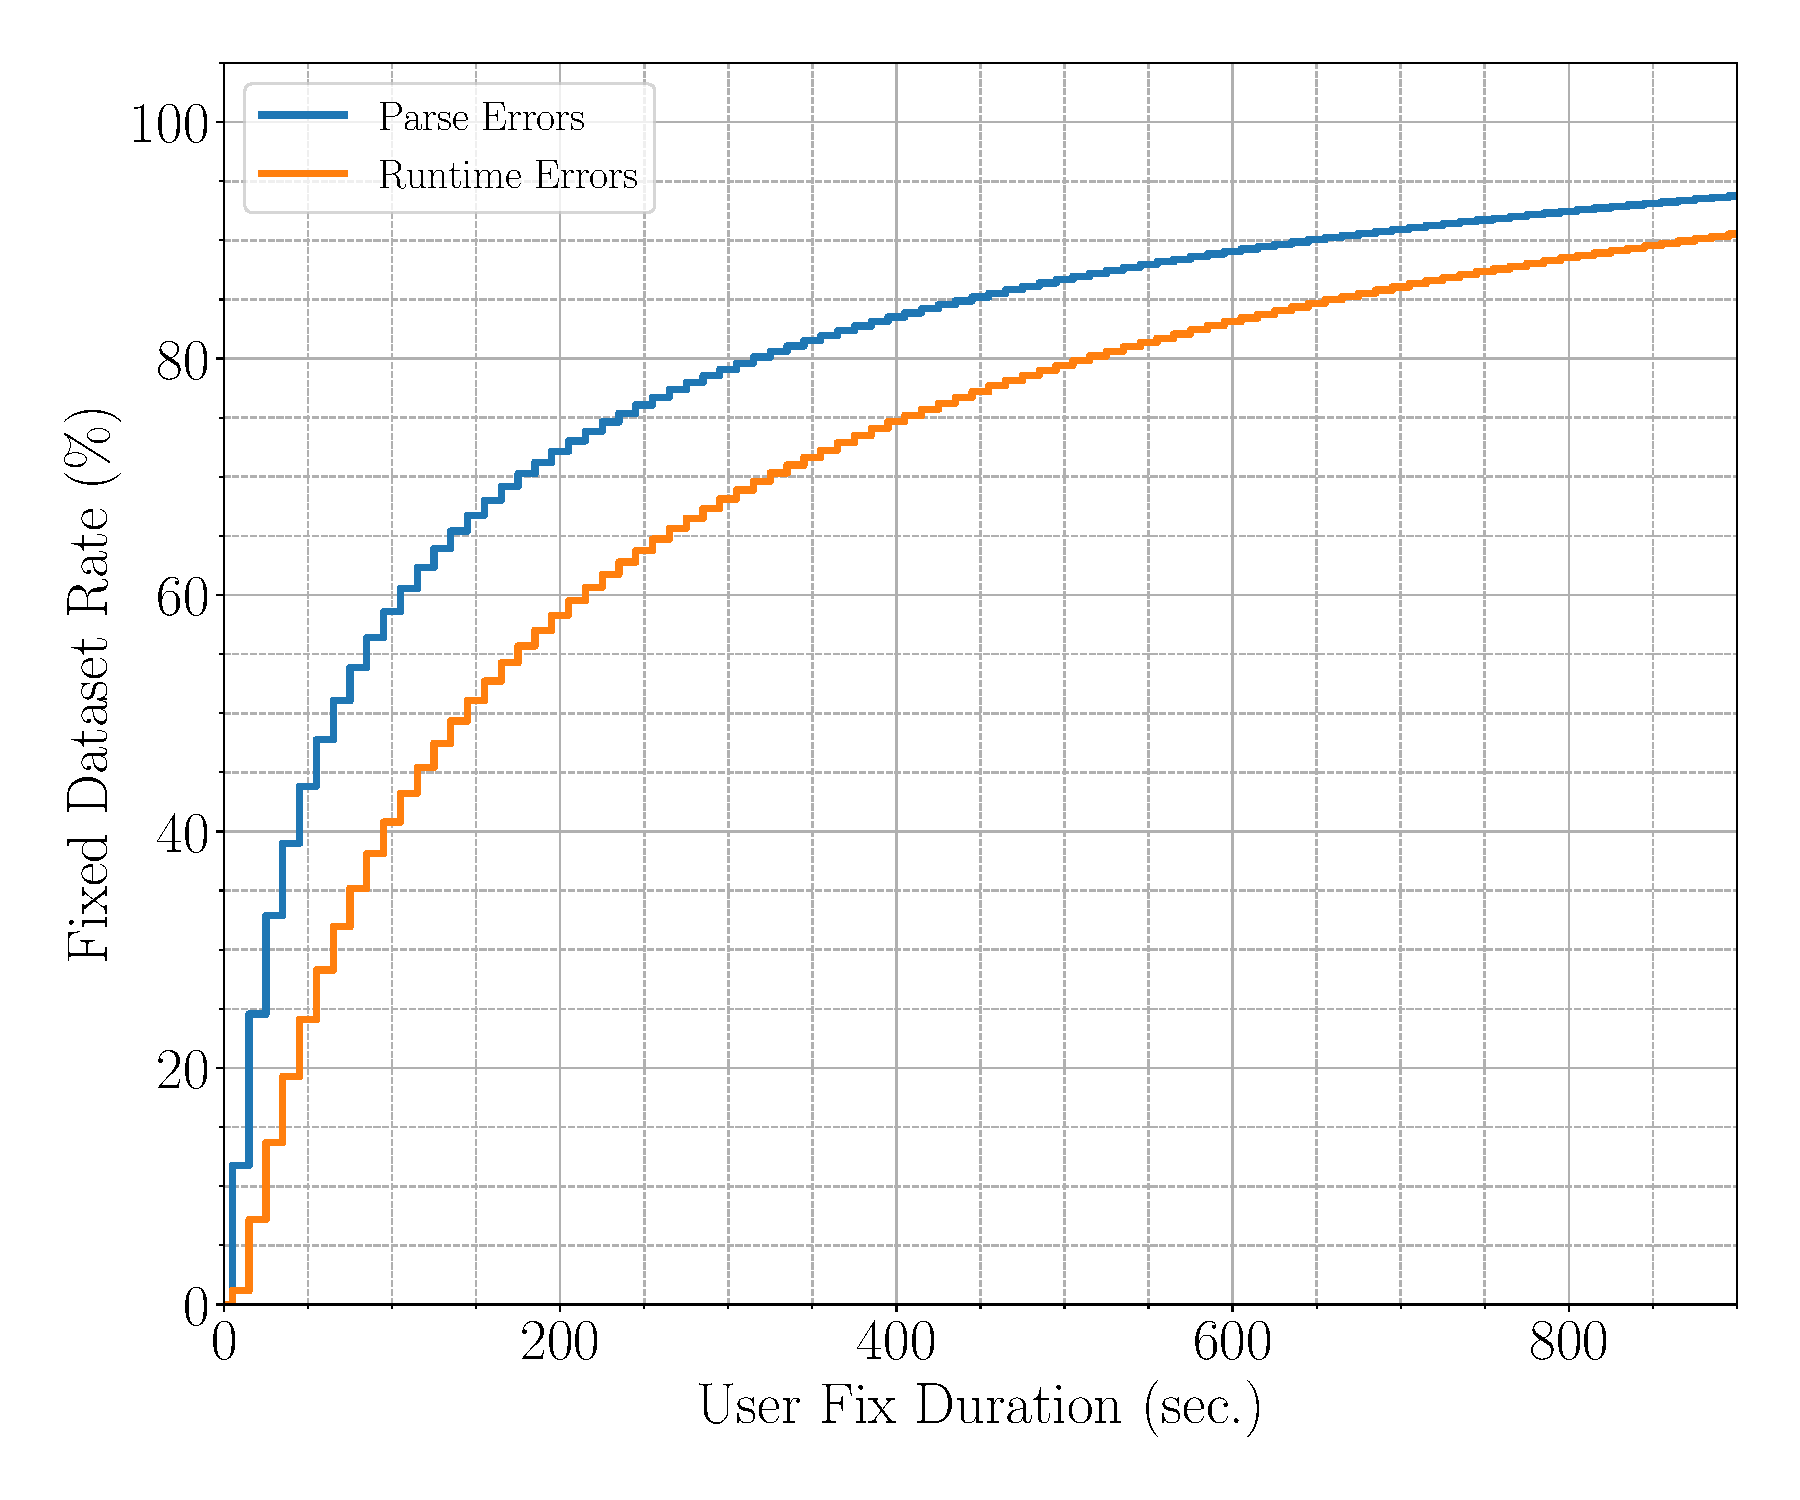
\includegraphics[width=\linewidth]{fixed-rate.pdf}
      \caption{The repair rates of the Python dataset.}
      \label{fig:repair-rate}
  \end{minipage}
\end{figure}

Parse errors (or \emph{Syntax Errors}) are usually easier to locate and repair
than other algorithmic or runtime errors \citep{Denny_2012}. For example, the
\emph{Python parser} will immediately inform the programmer for missing
parenthesis in function argument lists or for not having the proper indents in a
statement block. However, in this section we show that programmers (especially
novices) mostly deal with these kinds of errors on a daily basis and spend a
considerable amount of time fixing them, as has also be found in previous work
\citep{Ahadi_2018, Kummerfeld2003}.

\mypara{Parse errors are very common}
First of all, we count the different \emph{types} of errors users dealt with in
this dataset. \autoref{fig:error-statistics} presents the statistics of these
error types. We observe that $77.4 \% $ of all faulty programs in the dataset
failed with a syntax error. This accounts for the vast majority of the errors
that (novice) programmers face with their programs. The second category is
merely $13.6\%$ of the dataset and represents Python type errors. This is a
strong indication that these parse errors are very common and require an
automated approach of repairing.

\mypara{Parse errors take time to fix}
The web-based compiler that we used to generate our dataset, also provides us
with a \emph{server timestamp}. The timestamp is associated with each program
attempt submission, erroneous or not. The \emph{repair time} of an erroneous
program is calculated by taking the difference of the two timestamps of the
erroneous and fixed program. This method is not the most accurate metric of
repair time, since there are various reasons these timings are exaggerated, \eg
users stepping away from the computer, internet lag \etc. However, without loss
of generality, due to the large dataset of program repairs these timings can
still be viewed as an appropriate metric of the amount of time it took the
programmer to repair the errors in their program.

We plot in \autoref{fig:repair-rate} the \emph{programmer repair rate}, \ie the
dataset percentage that is repaired under a given amount of time. We present
here the repair rate for the parse errors and the rest of the errors grouped
together here as \emph{runtime} errors. As expected, the parse errors are fixed
faster than all the other ones, but not by a large difference. We observe for
example that within 2 minutes, usually $46\%$ of the runtime errors, \ie all the
errors that do not include the syntax errors, are repaired and around $63\%$ of
the syntax errors. Although, this is a considerable difference, we observe that
there is still a large number of the "simpler" parse errors that required more
than 2 minutes to be fixed. Therefore, we could conclude that an automated tool
that repairs (or parses) theses programs in only a few seconds could be
beneficial for a lot of programmers, novices or not.

\begin{figure}[t]
  \centering
  \begin{minipage}[c]{0.48\linewidth}
    \centering
    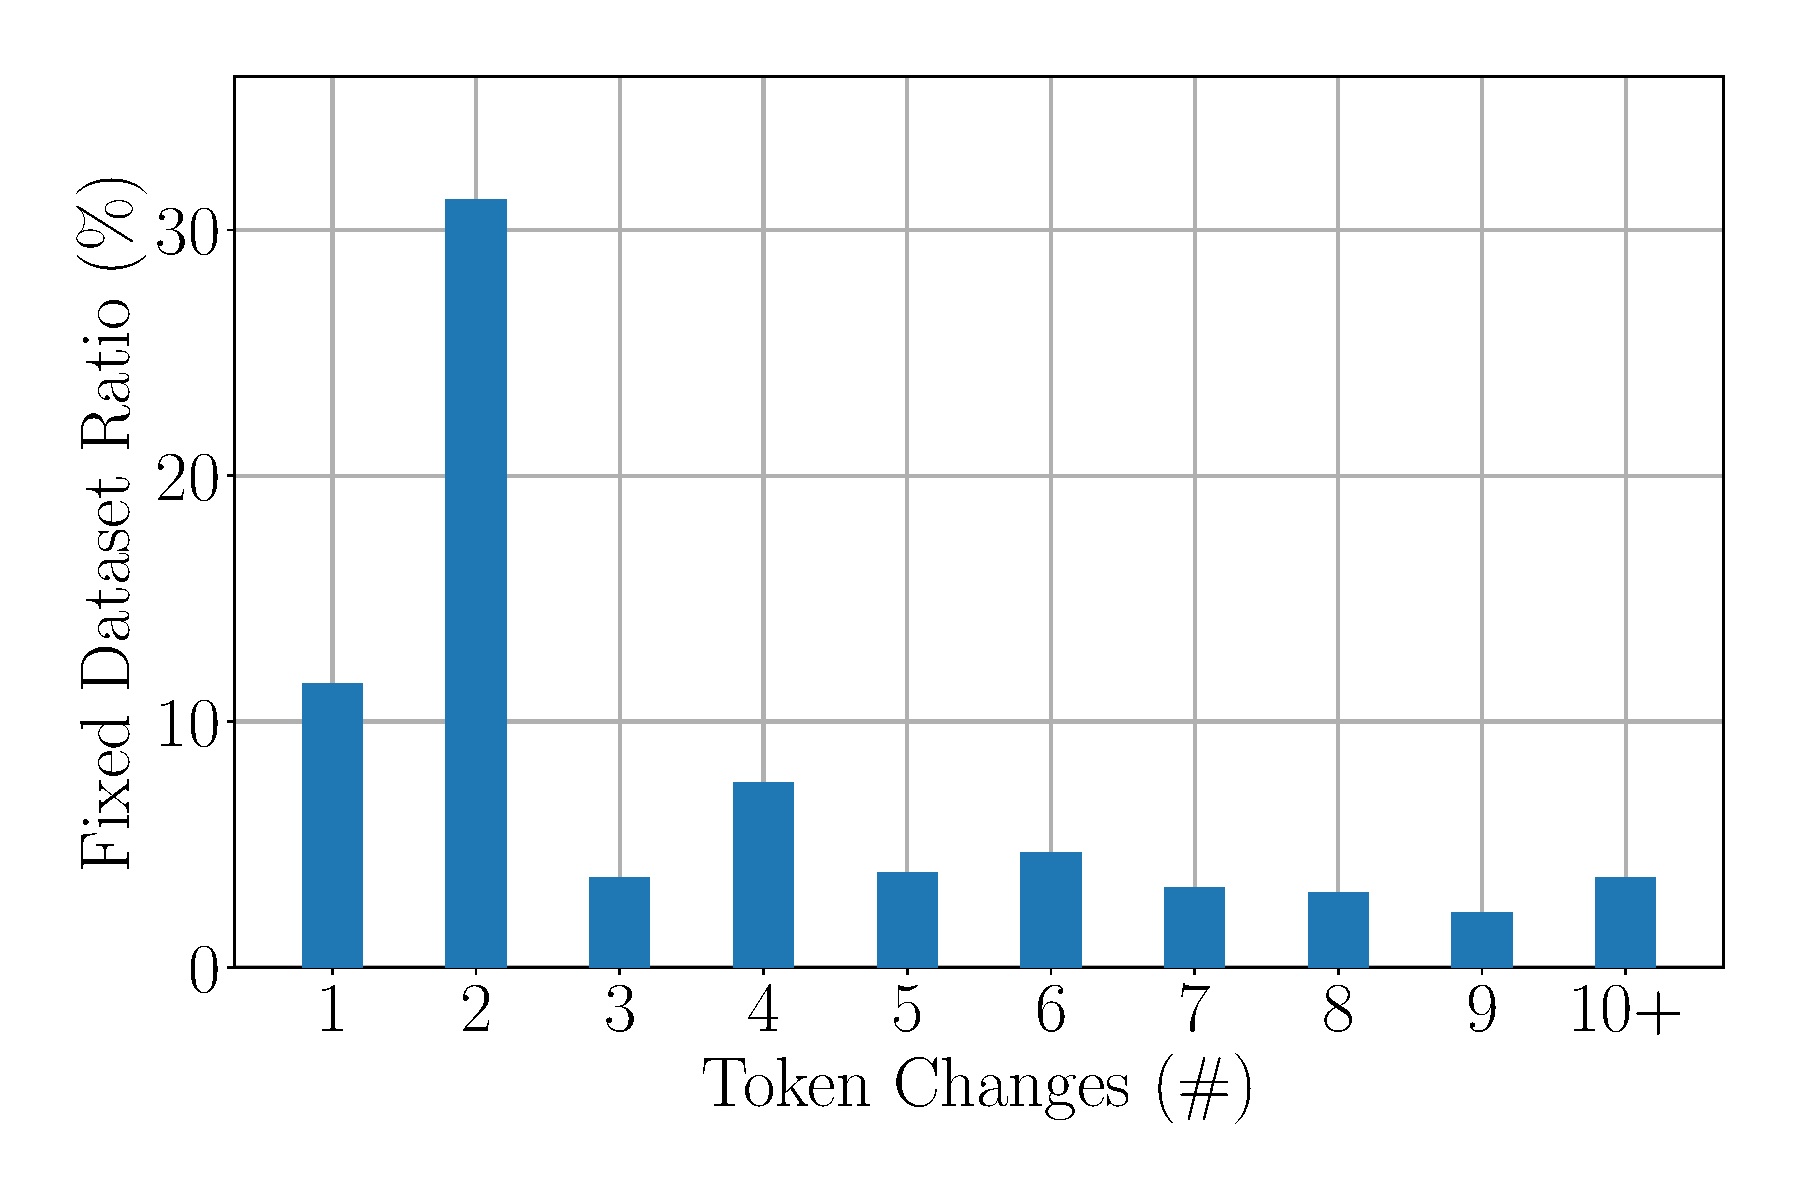
\includegraphics[width=\linewidth]{dataset-ratio-per-change.pdf}
    \caption{The Python dataset ratio that is fixed under the given number of
     token changes.}
    \label{fig:token-changes-ratio}
  \end{minipage}
  \hspace{0.02\linewidth}
  \begin{minipage}[c]{0.48\linewidth}
      \centering
      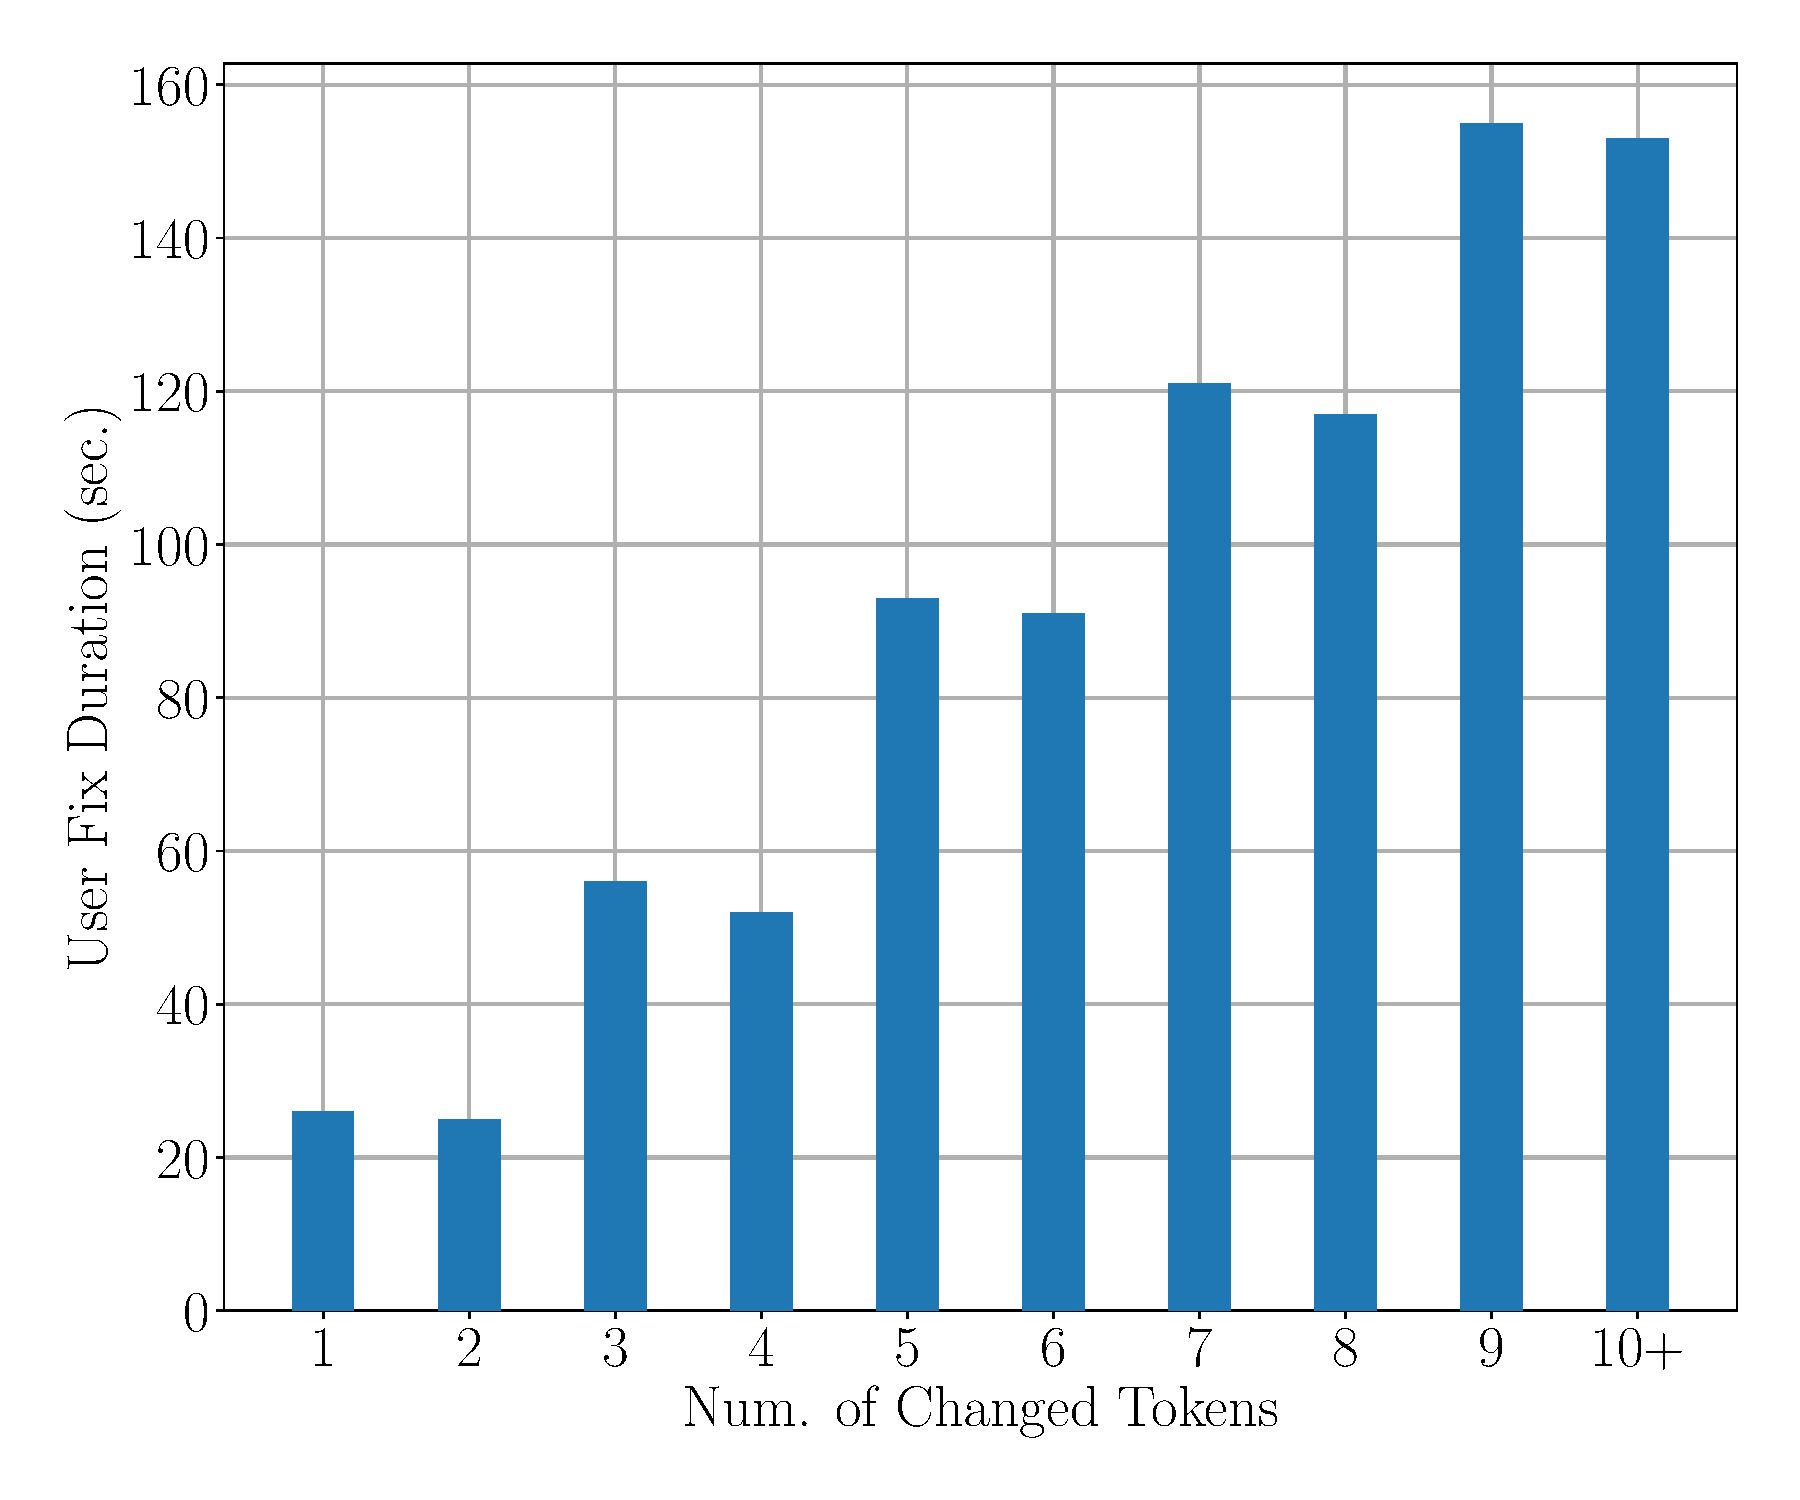
\includegraphics[width=\linewidth]{median-repair-times.pdf}
      \caption{The average time the user needed to fix the erroneous program
      for the needed token changes.}
      \label{fig:token-changes}
  \end{minipage}
\end{figure}

\mypara{Parse errors can require multiple edits to fix}
The average \emph{token-level changes} needed to fix a program with syntax
errors, \ie the number of changes in the lexed program token sequence, is
\emph{10.7 token changes}, while the \emph{median is 4}. A variable rename or a
different integer is not considered a change as they won't affect the syntax
error fix. As shown in \autoref{fig:token-changes-ratio}, $14.2\%$ of dataset
needs only one token change, $23.2\%$ needs two token changes, $7.0\%$ needs
three and $9.0\%$ needs four, \ie $53.4\%$ of the dataset needs at most 4 token
changes to be fixed. This shows that the majority of the syntax errors can be
fixed with only a few changes in their token sequences. But it is also important
to see how long it takes the users on average to make those changes.

\mypara{Parse errors with more edits take longer to fix}
\autoref{fig:token-changes} shows the average time that it takes a user to fix
their programs with syntax errors per the number of token-level changes in their
programs. As expected, with an increasing number of changes needed to fix all
parse errors, more time is needed for the programmers to make those changes.
Most importantly, even for one or two token changes the average user spends
\emph{26 and 25 sec} respectively, which is still a considerable amount of time
for these simple and short fixes. The repair time jumps to \emph{56 sec} for
three token changes.

These results further indicate that, while simple syntax errors can easily and
quickly be fixed by the programmers and the compiler error messages can be
helpful, programmers still struggle fixing programs that have more syntax
errors, that maybe the error message doesn't even point to.
